\documentclass[12pt]{article}
\usepackage[english,greek]{babel}
\usepackage[utf8x]{inputenc}
\usepackage{graphicx}
\usepackage{fullpage}
\begin{document}


\title{Έγγραφο Απαιτήσεων Λογισμικού $SRS$}
\date{\today}
\author{$Javengers$}

\maketitle

\tableofcontents

\section{Εισαγωγή}

\subsection{Σκοπός του Λογισμικού}

Σκοπός του παρόντος λογισμικού αποτελεί η πλήρης κατασκευή ενός ηλεκτρονικού παρατηρητηρίου τιμών που θα διευκολύνει και θα εμπλουτίζει την εμπειρία των καταναλωτών προσφέροντας τη δυνατότητα απλής και αποτελεσματικής αναζήτησς των τιμών που καταγράφονται για τα επιμέρους προϊόντα στα διάφορα μαγαζιά. Αξίζει να αναφερθεί, ότι η ηλεκτρονική μας πλατφόρμα θα βασίζεται στη μέθοδο του $crowdsourcing$, όπου δηλαδή ένα σύνολο από εγγεγραμμένους εθελοντές θα αποτελεί ενεργητικό κομμάτι της εφαρμογής και των προσφερόμενων υπηρεσιών πραγματοποιώντας καταχωρήσεις για προϊόντα και καταστήματα.

\subsection{Επισκόπηση Λογισμικού}

Η ιστοσελίδα μας υποστηρίζει τις ακόλουθες τρεις βασικές ομάδες χρηστών, που ενθυλακώνουν και τις επιμέρους λειτουργίες της εφαρμογής:
\begin{itemize}
\item Ο απλός χρήστης ή παρατηρητής που δεν έχει πραγματοποιήσει εγγραφή και του δίνεται η δυνατότητα να πραγματοποιεί αναζητήσεις στη βάση δεδομένων της εφαρμογής σχετικά με προϊόντα και τις αντίστοιχες καταχωρήσεις τους. Στο πλαίσιο αυτό, του δίνεται επίσης η δυνατότητα να φιλτράρει τα επιμέρους αποτελέσματα που προκύπτουν με βάση τις τιμές των καταχωρήσεων και την τοποθεσία των αντίστοιχων καταστημάτων.
\item Ο χρήστης εθελοντής που είναι σε θέση να εισάγει, να ανανεώνει και να διαγράφει δεδομένα σχετικά με τιμές των προϊόντων, των καταστημάτων και των καταχωρήσεων, συμμετέχοντας έτσι ενεργητικά στη σελίδα μας. Επιπλέον, του δίνεται η δυνατότητα να δημιουργήσει και να εμπλουτίσει ένα προφίλ που θα είναι διαθέσιμο και στους άλλους χρήστες, ενώ όπως γίνεται αντιληπτό είναι σε θέση να εκτελέσει τις ενέργειες ενός απλού μη εγγεγραμμένου χρήστη.
\item Ο δαιχειριστής της σελίδας, που έχει τον ρόλο του επιβλέποντα, επικοινωνεί και επεξεργάζεται τα αιτήματα των χρηστών ώστε να συντηρείται και να βελτιώνεται διαρκώς η σελίδα, ενώ είναι σε θέση να ελέγξει και να επεξεργαστεί τις καταχωρήσεις της βάσης δεδομένων με μία απλή διεπαφή. 
\end{itemize}

Με βάση λοιπόν τα παραπάνω, μπορούμε να συνοψίσουμε επιγραμματικά τις βασικές λειτουργικότητες που υποστηρίζονται που στη συνέχεια θα περιγράψουμε πιο αναλυτικά:

\begin{itemize}
\item Πλοήγηση στην αρχική σελίδα της εφαρμογής όπου αναγράφονται βασικές πληροφορίες σχετικά με την εξέλιξη της ιδέας μας
\item Αναζήτηση καταχωρήσεων και φιλτράρισμα των αποτελεσμάτων με βάση πολλαπλά κριτήρια
\item Επικοινωνία με τον διαχειριστή για να μεταφέρει σχόλια σχετικά με το $UX$
\item Δημιουργία Λογαριασμού και Σύνδεση στην Εφαρμογή
\item Πλοήγηση στο Dashboard του χρήστη και ανανέωση των πληροφοριών του που θα είναι διαθέσιμες και στους υπόλοιπους χρήστες
\item Εισαγωγή δεδομώνων σχετικά με προϊόντα, καταστήματα και καταχωρήσεις, καθώς και η αντίστοιχη ανανέωσή και διαγραφή τους
\end{itemize}

Οι παραπάνω δυνατότητες της ηλεκτρονικής μας πλατφόρμας θα γίνουν καλύτερα κατανοητές μέσα από μία σειρά από διαγράμματα $UML$. 

\newpage

\subsection{Διεπαφές με Εξωτερικά Συστήματα}

Όπως κάθε σύγχρονο έργο λογισμικού, η εφαρμογή μας επικοινωνεί, αλληλεπιδρά και αξιοποιεί μια πληθώρα από εξωτερικά λογισμικά, πόρους και βιβλιοθήκες για την αποδοτική και αποτελεσματική διεκπεραίωση των στόχων του λογισμικού. Για να γίνει καλύτερα κατανοητή η εξάρτηση αυτή, κρίνεται εύλογο να παρουσιάσουμε ένα διάγραμμα $UML-Deployment$, όπου αναπαριστώνται οι επιμέρους εξαρτήσεις της εφαρμογής μας με εξωτερικά συστήματα:

\begin{center}
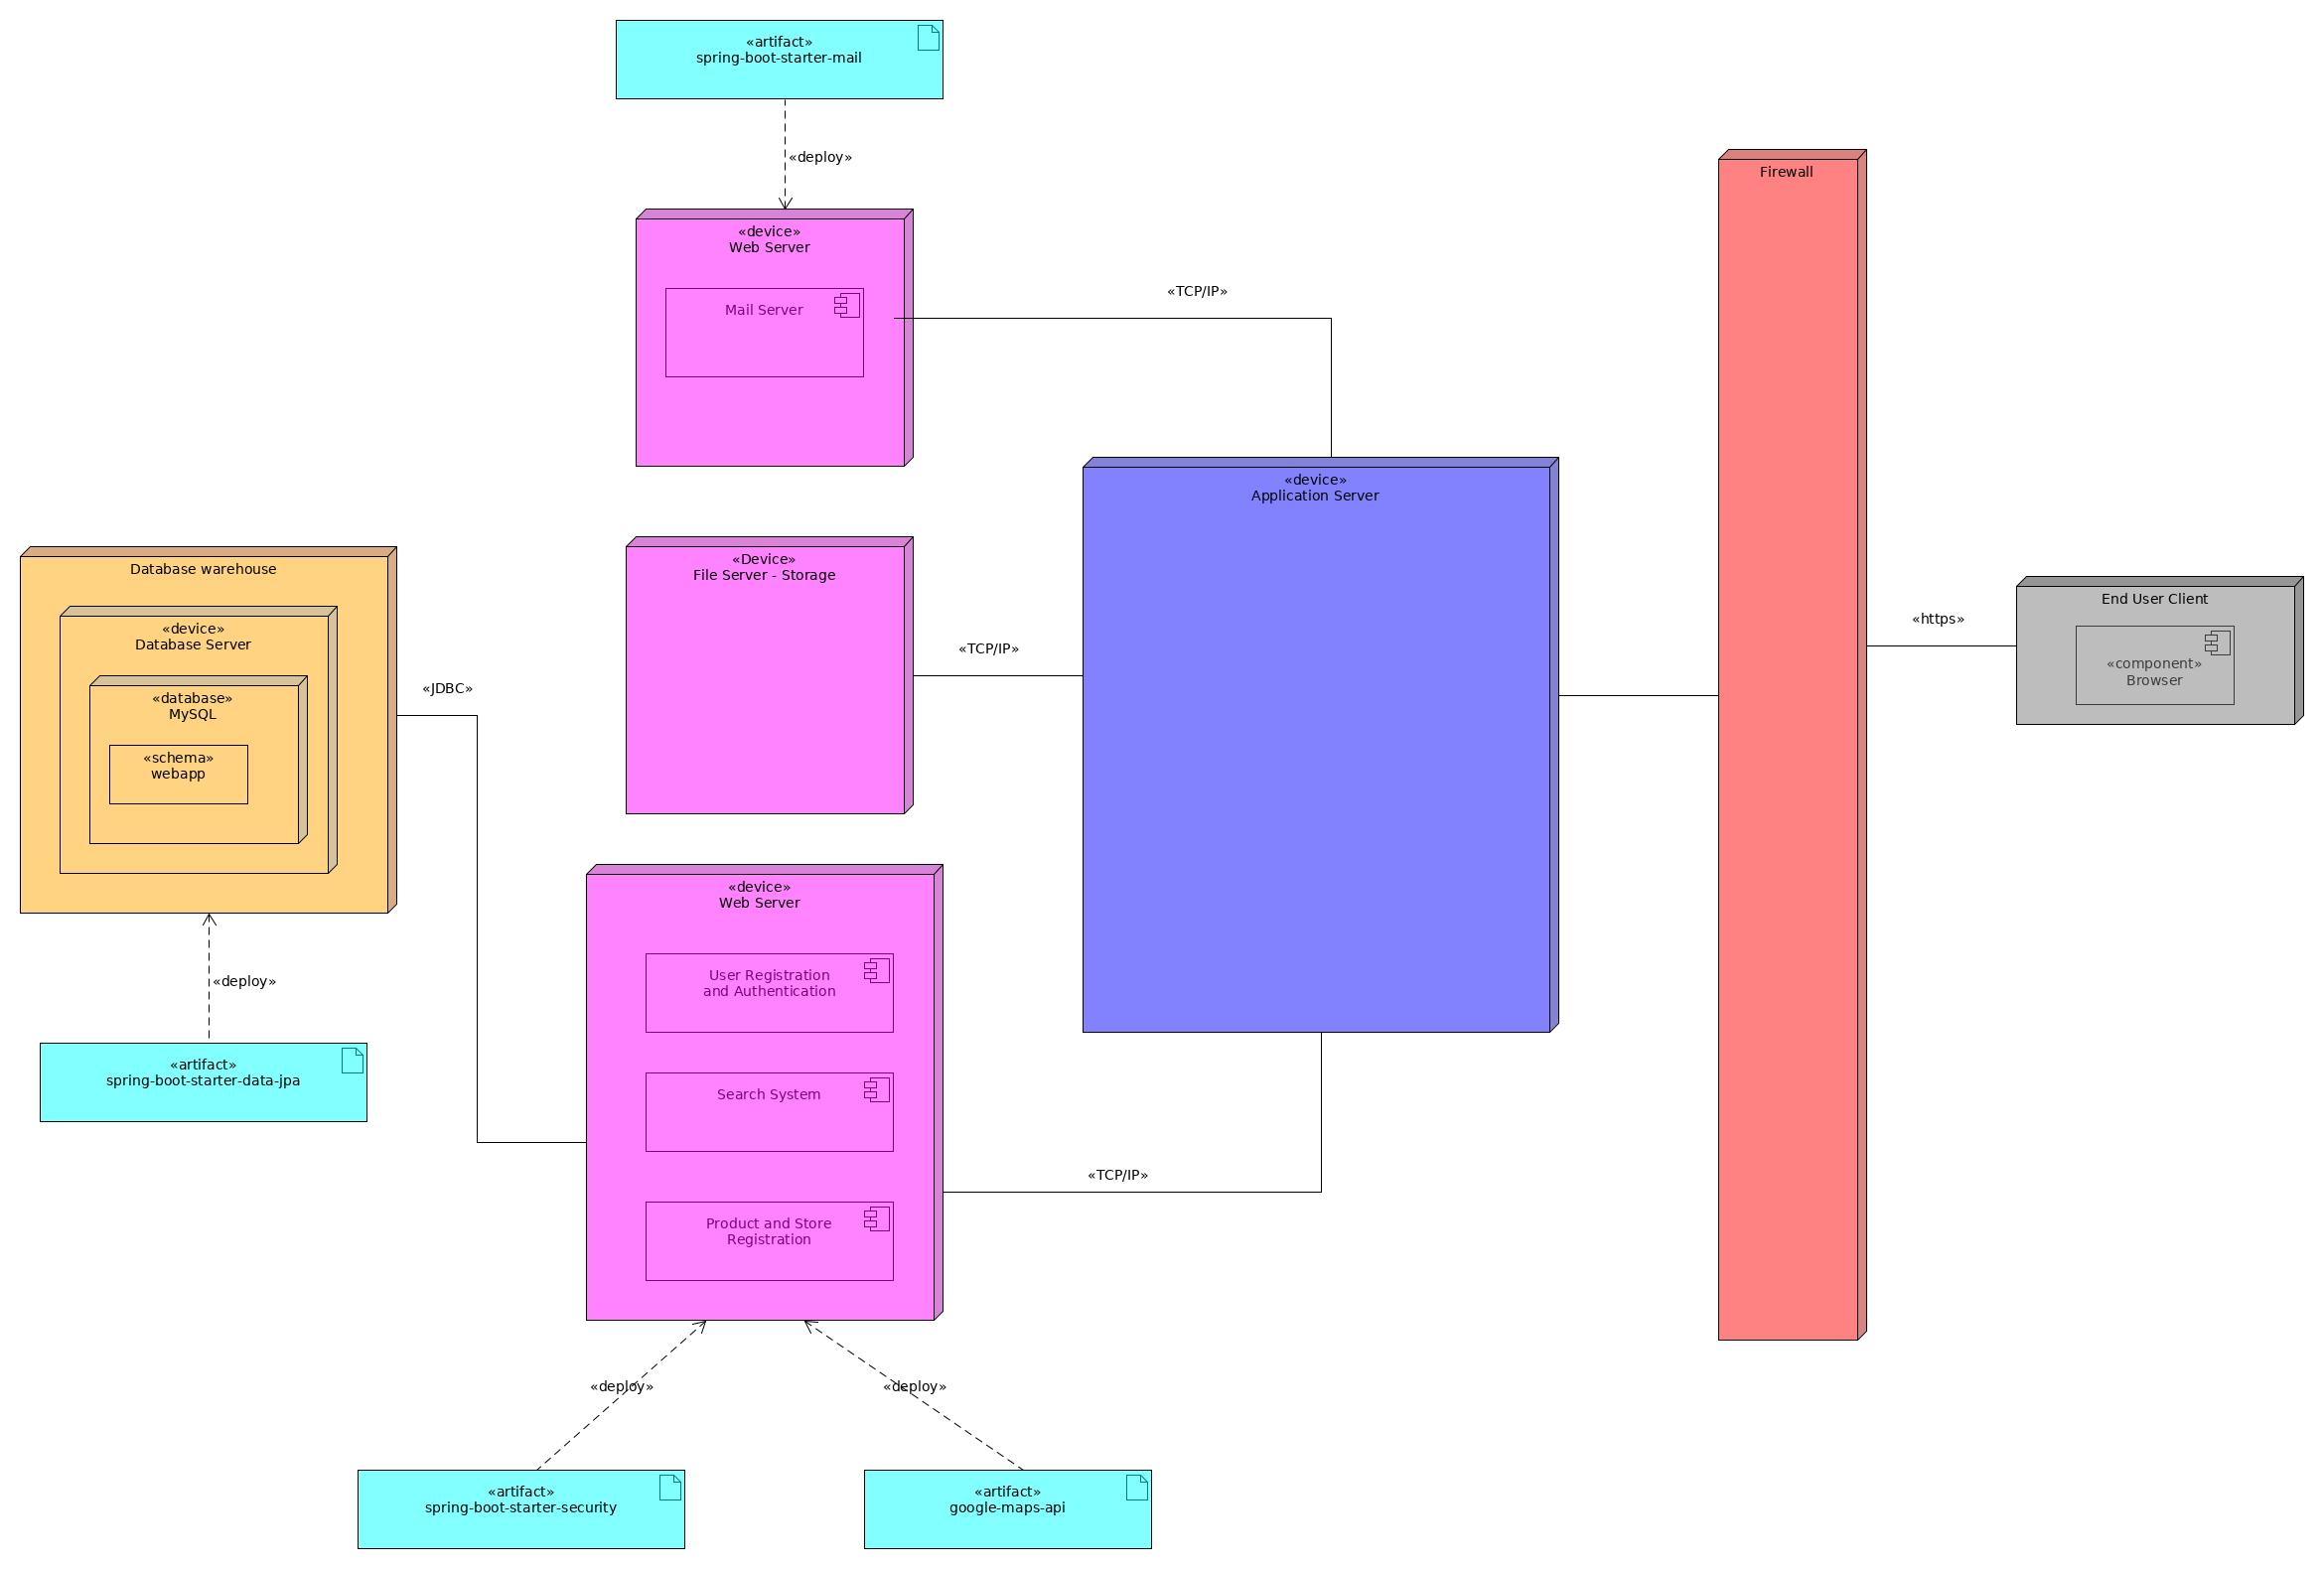
\includegraphics[scale=0.22]{UML/deploymentDiagram.jpg}
\end{center}

Το παραπάνω μοντέλο περιέχει και ορισμένους κόμβους που ενδεχομένως λόγω έλλειψης πόρων δεν θα είναι δυνατό να υλοποιθούν, αλλά αποτελεί ένα πιο γενικευμένο κατανεμημένο μοντέλο αρχιτεκτονικής για έργα λογισμικού μεγαλύτερης κλίμακας. Στα πλαίσια της δικής μας εφαρμογής, έχουμε χρησιμοποιήσει μία εικονική μηχανή που φιλοξενεί τη βάση δεδομένων μας, ώστε τα μέλη της ομάδας μας να έχουν κοινή αναφορά στα δεδομένα της εφαρμογής. Επιπλέον, από τις παραπάνω εξαρτήσεις αξίζει να επιμείνουμε στο $API$ της $Google$ που μας πρόσφερε μία διεπαφή για την αποτελεσματική εισαγωγή και αναζήτηση καταστημάτων σε χάρτες, δυνατότητα ιδιαίτερης σημασίας για την εφαρμογή μας.

\subsection{Διεπαφές με τον Χρήστη}

Για να οπτικοποιήσουμε καλύτερα τις διεπαφές που προφέρει η εφαρμογή μας με τους διάφορους χρήσετς και έχουμε ήδη αναφέρει παραθέτουμε το ακόλουθα διάγραμμα $UML$:

\begin{center}

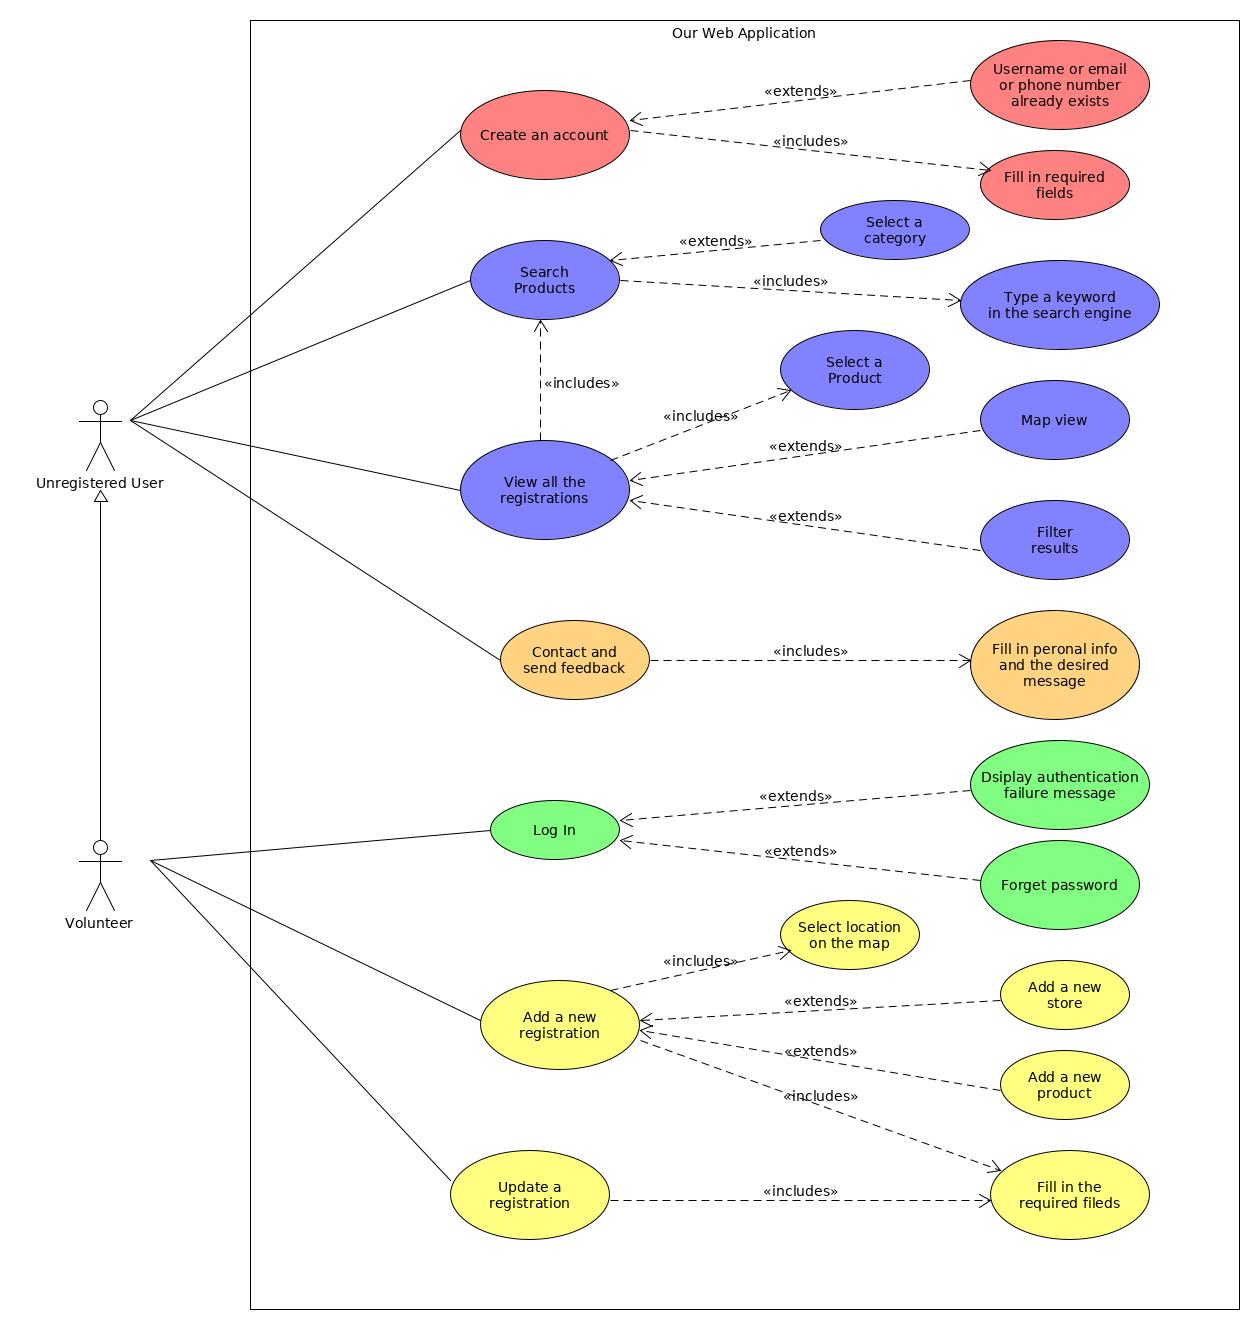
\includegraphics[scale=0.35]{UML/useCaseDiagram.jpg}

\end{center}

\section{Προδιαγραφές απαιτήσεων Λογισμικού}

\subsection{Λειτουργικές Απαιτήσεις}

Το παρών λογισμικό αποτελεί ένα ηλεκτρονικό παρατηρητήριο τιμών το οποίο χαρακτηρίζεται συνοπτικά από τις ακόλουθες βασικές λειτουργικότητες:

\begin{itemize}
\item Υποστήριξη διεπαφών χρήστη για αποτελεσματική αναζήτηση προϊόντων, των τιμών τους καθώς και του χωρικού αποτυπώματός τους, ενώ δίνεται ιδιαίτερη σημασία στην δυνατότητα παροχής ενός εύληπτου μηχανισμού σύγκρισης των επιμέρους καταχωρήσεων
\item Εγγραφή χρηστών στην υπηρεσία 
\item Εισαγωγή, Ανανέωση και Διαγραφή των επιμέρους καταχωρήσεων από τους εγγεγραμμένους χρήστες
\end{itemize}

Στο πλαίσιο αυτό, παρουσιάζουμε το ακόλουθο διάγραμμα $UML$ που απεικονίζονται τα επίμερους τμήματα που υποστηρίζουν τις βασικές λειτουργικές απαιτήσεις, σε υψηλό επίπεδο:

\begin{center}
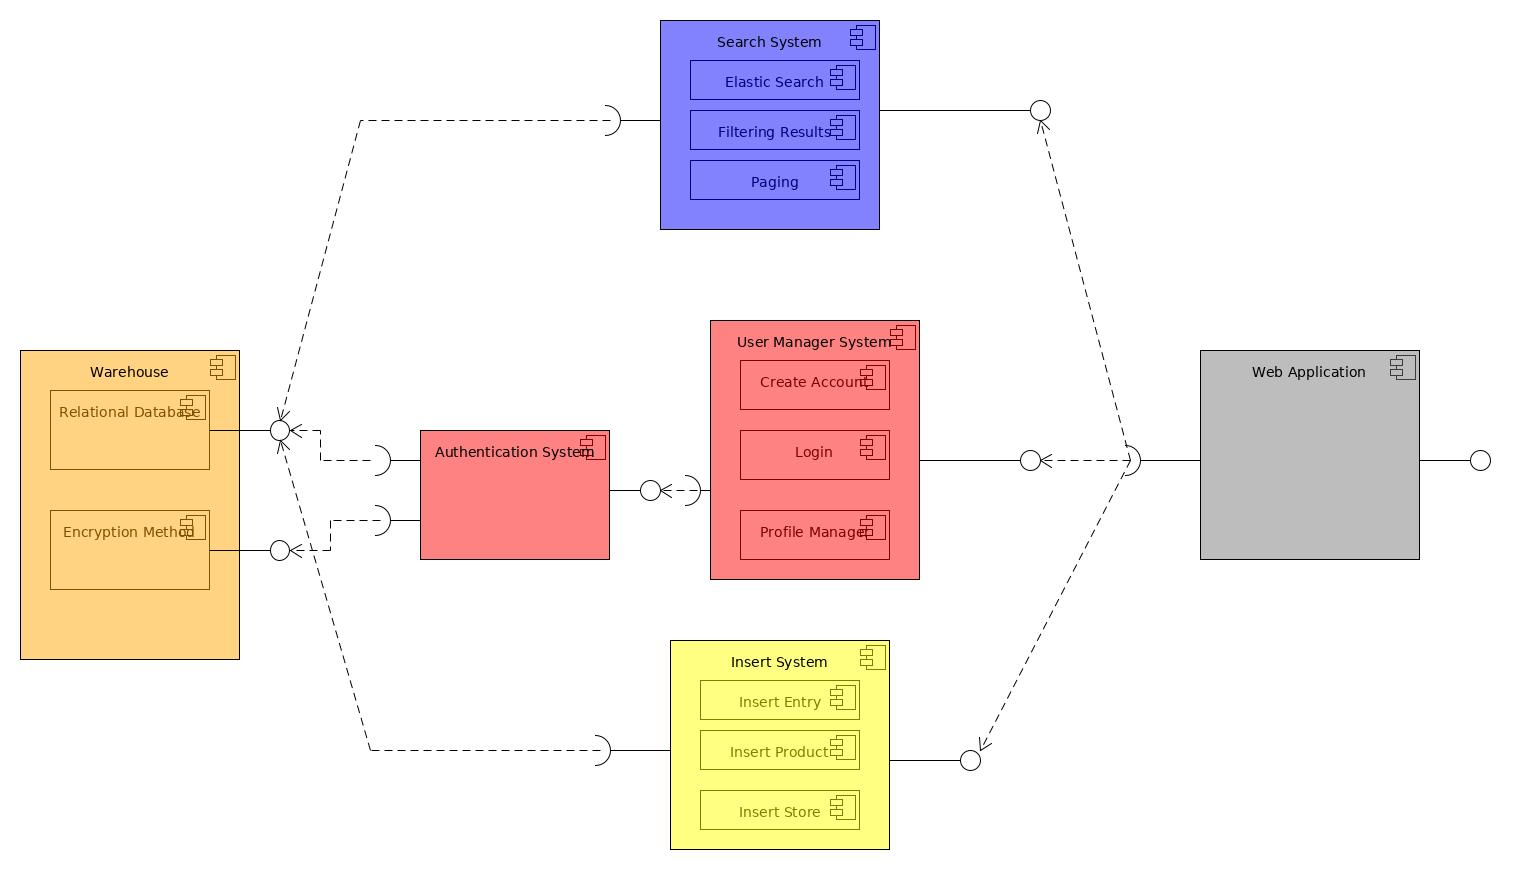
\includegraphics[scale=0.34]{UML/componentDiagram.jpg}
\end{center}

\newpage

\subsection{Μη Λειτουργικές Απαιτήσεις}

Επιπρόσθετα με τις παραπάνω απαιτήσεις, η επιτυχία της εφαρμογής μας εξαρτάται άμεσα και από την ικανοποίηση των παρακάτω προδιαγραφών:

\begin{itemize}
\item Απόδοση: Η ελαχιστοποίηση του χρόνου απόκρισης για τις αναζητήσεις που πραγματοποιεί ο χρήστης αλλά και συνολικά για τις επιμέρους ενέργειες που υποστηρίζονται από την πλατφόρμα. Για να το εφασφαλίσουμε αυτό έγινε χρήση κατάλληλων $indexes$ στη βάση δεδομένων για τη γρήγορη πραγαμτοποίηση $queries$, ενώ επίσης δόθηκε έμφαση στον σεβασμό των βασικών σχεδιαστικών αρχών που εξασφαλίζουν μεγαλύτερη απόδοση στην εφαρμογή
\item Ασφάλεια: Η προστασία των προσωπικών δεδομένων του χρήστη χρησιμοποιώντας μεθόδους κρυπτογράφησης, αλλά και η χρήση πρωτοκόλλων ασφαλής μεταφοράς δεδομένων ($https$). Συγκεκριμένα, χρησιμοποιήθηκε η μέθοδος $SaltPepper$, ενώ φροντίσαμε οι ευαίσθητες πληροφορίες των χρηστών, όπως είναι ο αριθμός τηλεφώνου, να μην είναι διαθέσιμες σε άλλους χρήστες
\item Διαθεσιμότητα: Η εξασφάλιση της διαρκής εύρυθμης λειτουργίας της ιστοσελίδας ανεξάρτητα από την ενδεχόμενη αποτυχία του δικτύου χρησιμοποιώντας κατανεμημένους $servers$. Στην περίπτωσή μας, χρησιμοποιήσαμε εικονικές μηχανές, ώστε στην περίπτωση αποτυχίας να υπάρχει $back-up$ εναλλακτική
\item Επεκτασιμότητα: Η οργάνωση και το στήσιμο της εφαρμογής με τέτοιο τρόπο που οι αλλαγές και οι επεκτάσεις των λειτουργικοτήτων να πραγματοποιούνται εύκολα και αποδοτικά
\item Απλότητα: Το σύνολο των διεπαφών που προσφέρει η εφαρμογή να ακολουθούν τις βασικές σχεδιαστικές αρχές της αλληλεπίδρασης ανθρώπου μηχανής
\item Κομψότητα: Η αισθητική πλευρά των διεπαφών του χρήστη
\end{itemize}



\section{Περιπτώσεις Χρήσης}

\subsection{Εγγραφή ενός Χρήστη}

\subsubsection{Ρόλοι που Εμπλέκονται}

Εμπλέκεται ο χρήστης που πραγματοποιεί την εγγραφή

\subsubsection{Προϋποθέσεις Εκτέλεσης}

Ο χρήστης θα πρέπει να συμπληρώσει τα απαιτούμενα πεδία με έγκυρες τιμές ανάλογα με το εκάστοτε πεδίο. Επίσης, στα πεδία $username$ , $email$ και $phone$ $number$ ο χρήστης απαιτείται να εισάγει μοναδικές τιμές που δεν υπάρχουν ήδη στη βάση.

\subsubsection{Περιβάλλον Εκτέλεσης}

Τα τμήματα που εμπλέκονται στη συγκεκριμένη περίπτωση χρήσης, είναι η διαδικτυακή διεπαφή της εφαρμογής μας για εγγραφή, καθώς και το σύστημα διαχείρισης βάσης που καλείται να πραγματοποιήσει και να ελέγξει την εγκυρότητα των εισαγομένων πεδίων.

\subsubsection{Δεδομένα Εισόδου}

\begin{itemize}
\item Ονοματεπώνυμο
\item $Username$
\item $Email$
\item Αριθμός Τηλεφώνου
\item Κωδικός Πρόσβασης
\end{itemize} 

\subsubsection{Παράμετροι}

\begin{itemize}
\item Ονοματεπώνυμο: Aαποτελείται αποκλειστικά από αλφαβητικούς χαρακτήρες
\item $Username$: Πρέπει να είναι μοναδικό για κάθε χρήστη
\item $Email$: Πρέπει επίσης να είναι μοναδικό ώστε κάθε διεύθυνση να αντιστοιχεί σε ένα χρήστη, ενώ ακολουθεί συγκεκριμένη δομή που ελέγχεται κατά την εισαγωγή του
\item Αριθμός τηλεφώνου: Οφείλει να είναι μοναδικό, ενώ είναι προαιρετικό πεδίο και αποτελείται από ακριβώς 10 ψηφία
\item Κωδικό  πρόσβασης: Πρέπει να αποτελείται από τουλάχιστον 10 χαρακτήρες
\end{itemize}

Αξίζει να αναφερθεί επίσης, ότι όλα τα παραπάνω πεδία έχουν το πολύ μέχρι 20 χαρακτήρες.

\subsubsection{Αλληλουχία Ενεργειών}

Η αλληλουχία των ενεργειών είναι η εξής:

\begin{enumerate}
\item Συμπλήρωση όλων των απαιτούμενων πεδίων
\item Επιλογή κουμπιού $submit$
\item Σε περίπτωση που δεν συμπληρώθηκαν κάποια πεδία σύμφωνα με τους παραπάνω περιορισμούς ο χρήστης πρέπει να συμπληρώσει ξανά σωστά τα πεδία για να ολοκληρωθεί η εγγραφή
\end{enumerate}

Πιο αναλυτικά και οπτικά, η παραπάνω διαδικασία παρουσιάζεται στο ακόλουθο $sequence$ $diagram$:


\begin{center}
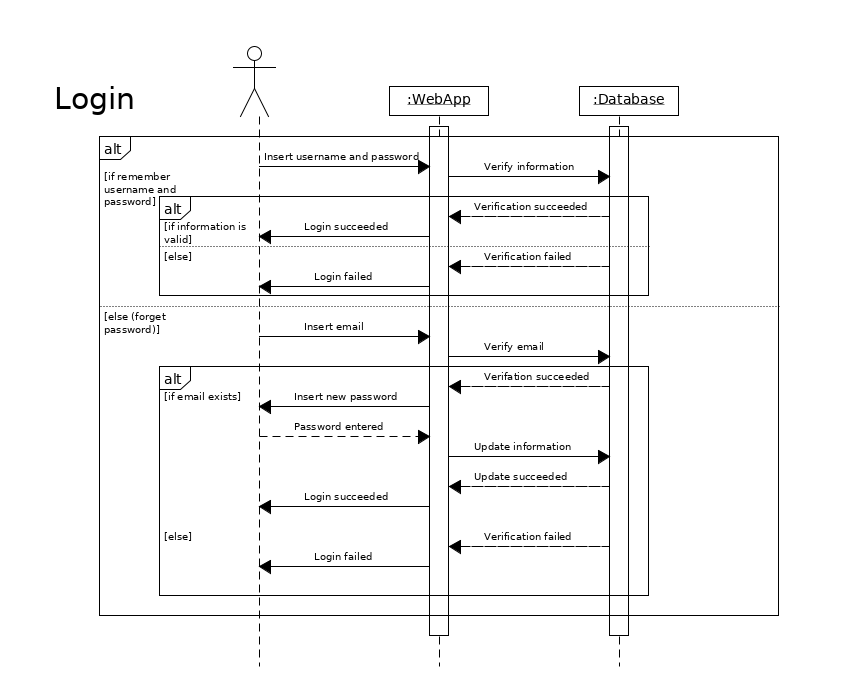
\includegraphics[scale=0.5]{UML/loginSequence.png}
\end{center}

\subsubsection{Δεδομένα Εξόδου}

Σε περίπτωση επιτυχημένης εγγραφής δημιουργείται ένας νέος χρήστης με τα αντίστοιχα χαρακτηριστικά και κατ' επέκταση μία νέα καταχώρηση στη βάση δεδομένων ενώ εμφανίζεται αντίστοιχο μήνυμα επιτυχίας στην οθόνη του χρήστη. Σε αντίθετη περίπτωση, εμφανίζεται μήνυμα αποτυχίας και παραμένει ο χρήστης στην ίδια οθόνη για να συμπληρώσει ο χρήστης τα στοιχεία σύμφωνα με τους περιορισμούς που έχουν επισημανθεί.


\subsection{Αναζήτηση Προϊόντος}

\subsubsection{Ρόλοι που Εμπλέκονται}

Εμπλέκεται και πάλι ένας χρήστης που είτε  είναι εγγεγραμμένος-εθελοντής, είτε είναι απλός επισκέπτης της σελίδας.
\subsubsection{Προϋποθέσεις Εκτέλεσης}

Ο χρήστης θα πρέπει είτε να συμπληρώσει ένα $keyword$ στη μηχανή αναζήτησς είτε να επιλέξει μία από τις καταγηροίες.

\subsubsection{Περιβάλλον Εκτέλεσης}

Τα τμήματα που εμπλέκονται στη συγκεκριμένη περίπτωση χρήσης, είναι η διαδικτυακή διεπαφή της εφαρμογής μας για αναζήτηση , καθώς και το σύστημα διαχείρισης βάσης που καλείται να πραγματοποιήσει την εύρεση των προϊόντων. 

\subsubsection{Δεδομένα Εισόδου}

Εισαγωγή κειμένου σχετικού με τις ετικέτες (tags) του προϊόντος που αναζητάμε ή επιλογή με τον κέρσορα της επιθυμητής κατηγορίας μέσα από τη διεπαφή που μας προσφέρει η σελίδα.

\subsubsection{Παράμετροι}

Οποιαδήποτε μορφή κειμένου δίνεται από το πληκτρολόγιο, χωρίς να ξεπεράσει τους 50 χαρακτήρες

\subsubsection{Αλληλουχία Ενεργειών}

Η αλληλουχία των ενεργειών περιλαμβάνει είτε την είσοδο δεδομένων από τη μηχανή αναζήτησης είτε την επιλογή κάποιας κατηγορίας και παρουσιάζεται παρακάτω πιο αναπαραστατικά στο ακόλουθο $sequence$ $diagram$:


\begin{center}
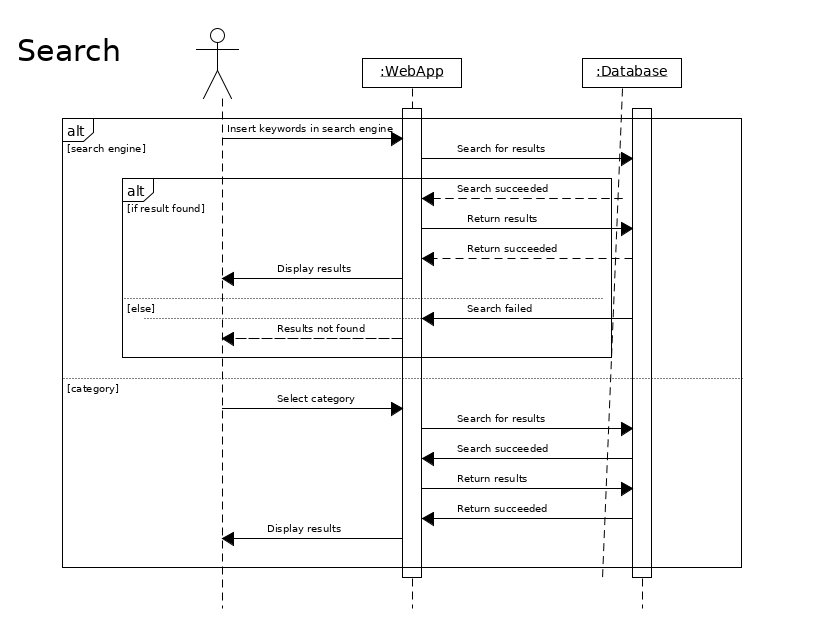
\includegraphics[scale=0.5]{UML/searchSequence.png}
\end{center}

\subsubsection{Δεδομένα Εξόδου}

Λίστα με τα προϊόντα με βάση τα πεδία αναζήτησης. Σε περίπτωση που δεν υπάρχουν αποτελέσματα αναζήτησης εμφανίζεται σχετικό μηνύμα.


\subsection{Προσθήκη Νέα Καταχώρησης}


\subsubsection{Ρόλοι που Εμπλέκονται}

Η προσθήκη νέου προϊόντος μπορεί να πραγματοποιηθεί μόνο από εθελοντή, δηλαδή από έναν χρήστη που έχει πραγματοποιήσει εγγραφή στην υπηρεσία.

\subsubsection{Προϋποθέσεις Εκτέλεσης}

Ο χρήστης θα πρέπει να συμπληρώσει τα απαιτούμενα πεδία με έγκυρες τιμές ανάλογα με το εκάστοτε πεδίο. 

\subsubsection{Περιβάλλον Εκτέλεσης}

Τα τμήματα που εμπλέκονται στη συγκεκριμένη περίπτωση χρήσης, είναι η διαδικτυακή διεπαφή της εφαρμογής μας για προσθήκη νέας καταχώρησης , καθώς και το σύστημα διαχείρισης βάσης που καλείται να πραγματοποιήσει την νέα καταχώρηση ελέγχοντας αν τα δεδομένα εισόδου(προϊόν ή κατάστημα) υπάρχουν ήδη στη βάση. 

\subsubsection{Δεδομένα Εισόδου}

Ο χρήστης καλείται να εισάγει τις ακόλουθες πληροφορίες:

\begin{itemize}
\item $Barcode$
\item Ετικέτες
\item Αξιολόγηση
\item Ετικέτες
\item Όνομα καταστήματος
\item Τοποθεσία καταστήματος
\item Τιμή προϊόντος
\end{itemize}

Αν το $barcode$ δεν υπάρχει στη βάση δεδομένων, ζητείται από την εθελοντή να κάνει την εισαγωγή του νέου προϊόντος εισάγοντας και τα εξής χαρακτηριστικά:

\begin{itemize}
\item Όνομα προϊόντος
\item Κατασκευαστής
\item Κατηγορία
\item Εικόνα προϊόντος
\item Περιγραφή προϊόντος
\end{itemize}

\subsubsection{Παράμετροι}

Τα παραπάνω δεδομένα εισόδου χαρακτηρίζονται από τους εξής περιορισμούς:

\begin{itemize}

\item Τιμή Προϊόντος: Είναι αριθμός διπλής ακρίβειας με περιορισμό δυο δεκαδικών ψηφίων

\item $Barcode$: Περιέχει το πολύ 20 χαρακτήρες

\item Όνομα καταστήματος: Αποτελείται από αλφαριθμητικούς χαρακτήρες

\item Τοποθεσία καταστήματος: Η εισαγωγή της θα γίνει εισάγοντας τη διεύθυνση ή επιλέγοντας την τοποθεσία του στο χάρτη

\item Ετικέτες: Αποτελούνται από χαρακτήρες χωρίς κενά διαστήματα

\item Αξιολόγηση: Aριθμός από 0.5 μέχρι 5.0 με βήμα 0.5

\item Όνομα προϊόντος: Aποτελείται από αλφαριθμητικούς χαρακτήρες

\item Κατασκευαστής: Aποτελείται από αλφαριθμητικούς χαρακτήρες

\item Κατηγορία: Aποτελείται από αλφαριθμητικούς χαρακτήρες

\item Εικόνα Προϊόντος: Έγκυρο $URL$ εικόνας
\item Περιγραφή προϊόντος: Οποιαδήποτε μορφή κειμένου κρίνει ο χρήστης ότι απαιτείται για να περιγράψει το προϊον
\end{itemize}

\subsubsection{Αλληλουχία Ενεργειών}

Η αλληλουχία των ενεργειών περιλαμβάνει τις ακόλουθες ενέργειες:

\begin{itemize}
\item Εισαγωγή $barcode$, ενώ αν δεν υπάρχει ήδη στη βάση καλείται να συμπληρώσει τα πεδία που σχετίζονται με το προϊόν
\item Εισαγωγή αξιολόγησης και ετικετών για το προϊόν
\item Εισαγωγή τοποθεσίας καταστήματος, ονόματος καταστήματος καθώς και τιμής του προϊόντος
\end{itemize}

Η παραπάνω αλληλουχία γίνεται καλύτερα κατανοητή μέσα από το παρακάτω διάγραμμα $UML$:

\begin{center}
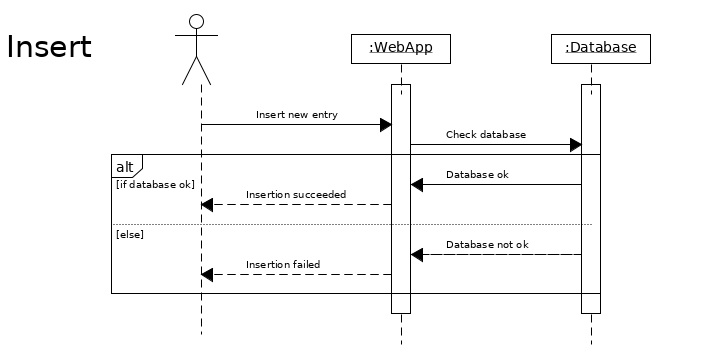
\includegraphics[scale=0.5]{UML/insertSequence.png}
\end{center}

\subsubsection{Δεδομένα Εξόδου}

Εμφανίζεται κατάλληλο μήνυμα που επιβεβαιώνει ότι η καταχώρηση ήταν επιτυχής, ενώ ο χρήστης μεταφέρεται εκ νέου στη σελίδα προφίλ.

\subsection{Απαιτήσεις Επιδόσεων}

Για να θεωρείται επιτυχημένη η εφαρμογή μας και η διεπαφή μας ενδιαφέρει ο χρόνος που απαιτείται για την πραγματοποιήση μιας καταχώρησης, ο αριθμός των λαθώς που γίνονται από τη μεριά του χρήστη καθώς και η ικανοποίηση που λαμβάνει ο χρήστης από τη χρησιμοποίηση της διεπάφης. 


\subsection{Απαιτήσεις Οργάνωσης Δεδομένων}

\subsubsection{Τεχνική Περιγραφή των Δεδομένων}

Για την αποδοτική αποθήκευση, διαχείριση  και ανάκτηση των δεδομένων που εισάγονται από τη εφαρμογή έχει χρησιμοποιηθεί μία Σχεσιακή βάση δεδομένων και συγκεκριμένα το σύστημα διαχείρισης $MySQL$. Στο πλαίσιο αυτό, οι περιορισμοί που έχουμε ήδη αναφέρει και ελέγχονται στο $front-end$ μέσα από τις διάφορες φόρμες πρέπει να είναι συνεπείς με τους περιορισμούς της βάσης δεδομένων, καθώς ένας κακόβουλος χρήστης θα μπορούσα να πραγματοποιήσει εισαγωγές παρακάπτοντας τις φόρμες, δημιουργώντας με αυτόν τον τρόπο ασυνέπειες στη βάση μας. Δηλαδή, κάθε εισαγωγή ή ανανέωση είναι ευθυγραμμισμένη με τους περιορισμούς που έχουμε ήδη αναφέρει. Όπως γίνεται αντιληπτό, σχετικά με τα πρότυπα των δεδομένων έχουν χρησιμοποιηθεί τα καθιερωμένα που σχετίζονται με σχεσιακές βάσεις δεδομένων και συγκεκριμένα με την $MySQL$. 

\subsubsection{Απαιτήσεις και Περιορισμοί Πρόσβασης στα Δεδομένα}

Κάθε χρήστης μπορεί να δει τα προσωπικά δεδομένα που έχει δημοσιεύσει ένας άλλος εγγεγραμμένος χρήστης στο προφίλ του, εκτός από ευαίσθητες πληροφορίες όπως ο αριθμός τηλεφώνου και φυσικά ο κωδικός πρόσβασης. Από την άλλη, οι πληροφορίες που σχετίζονται με τις καταχωρήσεις προϊόντων και καταστημάτων είναι διαθέσιμες χωρίς περιορισμούς, ενώ πρέπει να αναφερθεί ότι αν και ο διαχειριστής του συστήματος έχει πρόσβαση στην ολότητα της πληροφορίας στη βάση δεδομένων, δεν έχει πρόσβαση στον κωδικό του εκάστοτε χρήστη καθώς είναι κρυπτογραφημένος.

\subsubsection{Μοντέλο Δεδομένων}

Για να δείξουμε τη δομή στην οποία βασίζεται το μοντέλο τη εφαρμογής παραθέτουμε το ακόλουθο διάγραμμα $UML$:

\begin{center}
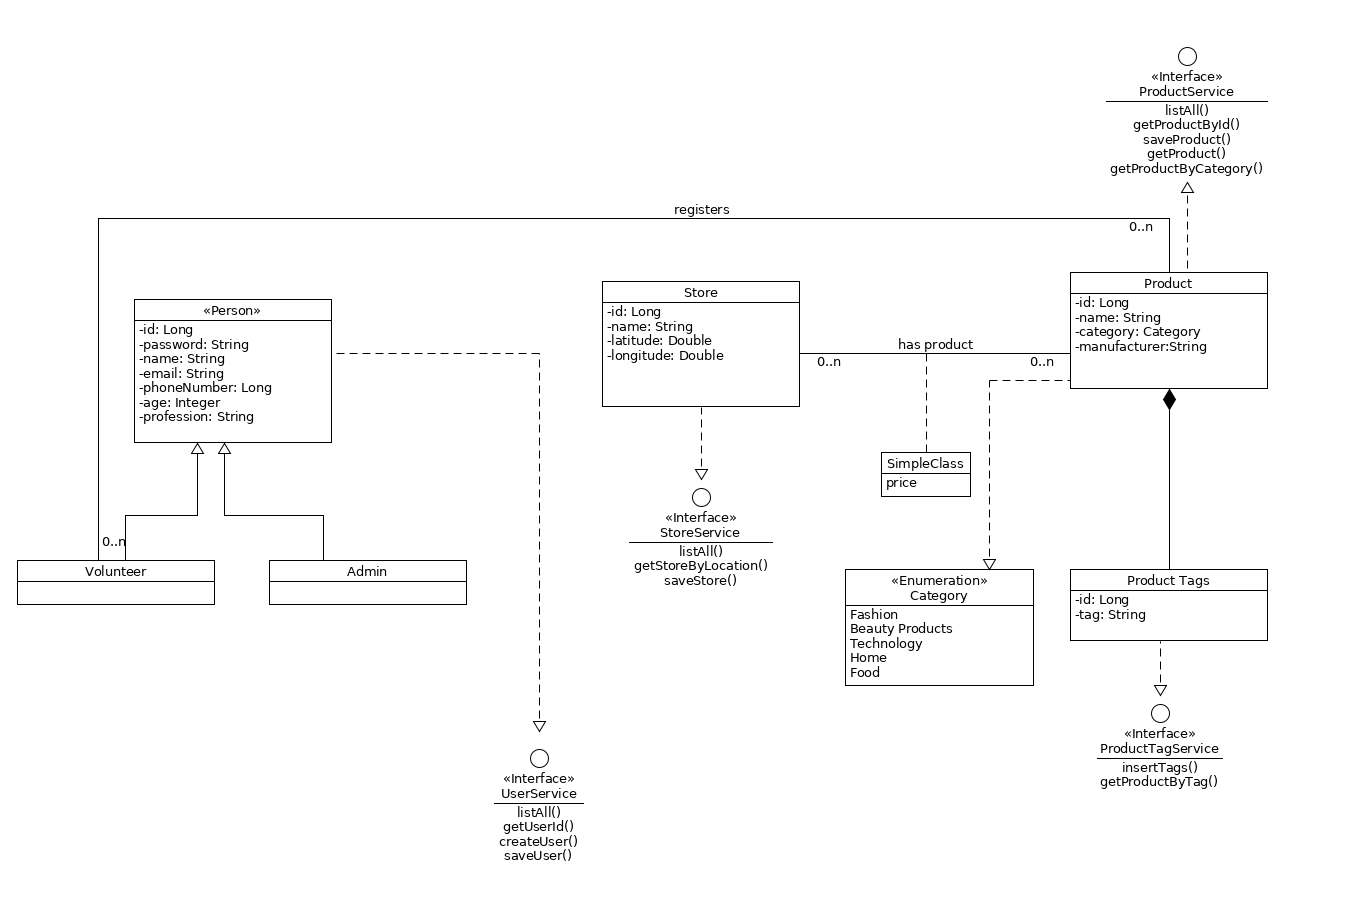
\includegraphics[scale=0.35]{UML/classDiagram.png}
\end{center}


\subsubsection{Προδιαγραφές Ακεραιότητας Δεδομένων}

Στη βάση δεδομένων έχουν χρησιμοποιηθεί οι κανόνες ακεραιότητας των δεδομένων που σχετίζονται με τις εξαρτήσεις των επιμέρους οντοτήτων, δηλαδή με $foreign-key-constraints$. Συγκεκριμένα, η προδιαγραφή αυτή επιτυγχάνεται με τη χρήση $foreign-keys$ και με ενέργειες όπως το $on-delete-casacde$, ώστε τα δεδομένα της βάσης μας να είναι συνεπή. Επιπλέον, οι προδιαγραφές ακεραιότητας επιτυγχάνονται χρησιμοποιώντας κατάλληλα $triggers$ ώστε να ικανοποιούνται οι περιορισμοί που αναφέρθηκαν αλλά και να ικανοποιηθεί η απαίτησεις για $ACID-Transactions$


\subsubsection{Προδιαγραφές Διατήρησης Δεδομένων}

Για την διατήρηση δεδομένων μπορούμε να αναφέρουμε μεθόδους όπως η $RAID-V$ για την ασφάλιση των δεδομένων στην περίπτωση που αποτύγχει ένας δίσκος καθώς και την πολλαπλή αντιγραφή των κρίσιμων δεδομένων της εφαρμογής.

\subsection{Περιορισμοί Σχεδιάσης}

Σχετικά με τους περιοσιμούς σχεδίασης ακολουθήσαμε το τυπικό πρότυπο που ακολουθείται κατά τον προγραμματισμό σε $Java$. Η συμμόρφωση στα πρότυπα αυτά αν και δεν είναι είναι υποχρεωτική μας βοηθάει να διατηρούμε ευανάγνωστο τον κώδικα για όλα τα μέλη της ομάδας, καθώς και για άλλα εξωτερικά άτομα. Οι βασικοί κανόνες είναι οι ακόλουθοι:

\begin{itemize}
\item Τα ονόματα Κλάσεων ξεκινούν με κεφαλαία γράμματα και ακολουθούν $camel-case$
\item Το ονόματα πεδίων σε Κλάσεις ξεκινούν με πεζό γράμμα, ενώ ακολουθούν επίσης $camel-case$.
\item Τα ονόματα των $packages$ ξεκινούν με μικρό γράμμα, ενώ σε περίπτωση που αποτελούνται από πολλές λέξεις χωρίζονται από τελείες. 
\end{itemize}

\subsection{Λοιπές Απαιτήσεις}

\subsubsection{Απαιτήσεις Διαθεσιμότητας}

Όπως έχει ήδη αναφερθεί, για να εξασφαλίσουμε τη διαθεσιμότητα θα πρέπει το σύστημα να επικοινωνεί με πολλαπλούς $database$ $servers$, ώστε να υπάρχουν πολλαπλά αντίγραφα για τη βάση δεδομένων σε διαφορεικούς παρόχους. Επίσης, θα πρέπει να συνεργαζόμαστε με παρόχους που μα εξασφαλίζουν 99.99\% διαθεσιμότητα διαδικτυακής σύνδεσης μέσω των υποδομών τους.

\subsubsection{Απαιτήσεις Ασφάλειας}

Οι απαιτήσεις ασφάλειας συνοψίζονται στα ακόλουθα σημεία:

\begin{itemize}
\item Το σύστημα θα χρησιμοποιεί ασφαλή $sockets$ σε όλες τις ανταλλαγές ευαίσθητων δεδομένων του χρήστη
\item Το σύστημα θα αποσυνδέει αυτόματα τους χρήστες μετά από μια περίοδο αδράνειας

\item Το σύστημα δεν θα προβάλει ποτέ τον κωδικό του χρήστη κατά την πληκτρολόγηση, αλλά θα χρησιμοποιεί αντ' αυτού ειδικούς κωδικοποιημένους χαρακτήρες.
\item Οι κωδικοί των χρηστών θα αποθηκεύονται στη βάση δεδομένων κρυπτογραφημένοι ώστε ακόμα και σε περίπτωση που ένας κακόβουλος χρήστης αποκτήσει πρόσβαση στη βάση μας, δε θα είναι σε θέση να ανιχνεύσει τον πραγματικό κωδικό.
\item Ο $server$ του συστήματος θα είναι προσβάσιμος μονάχα από επικυρωμένους διαχειριστές.
\end{itemize}

\subsubsection{Απαιτήσεις Συντήρησης}

Ο πηγαίος κώδικος που αντιστοιχεί στην εφαρμογή θα πρέπει να περνάει από τακτικούς ελέγχους και να αναθεωρείται με βάση και τις απαιτήσεις και την αλληλεπίδραση των χρηστών.

\end{document}